%\makeatletter
%\def\toclevel@chapter{0}
%\makeatother


\chapter{Approche spectrale}
%\begin{tikzpicture}[remember picture, overlay]
%\node[anchor=north east,inner sep=0pt] at (current page.north east) {
\includegraphics[scale=1]{Fig/Chapter1/g825.png}};
%\end{tikzpicture}
\label{ch:TauS_NJP}

Dans le chapitre précédent, nous nous sommes concentrés sur la mesure du temps de diffusion élastique, que nous avons comparé à la théorie perturbative de Born. En particulier, nous avons montré que celle-ci fournit une prédiction quantitative du temps de diffusion élastique dans le régime de diffusion faible, mais que de fortes déviations apparaissent lorsque l'amplitude du désordre $|\VR|$ augmente et que l'impulsion initiale $k_{\mathrm{i}}$ diminue. La comparaison de nos données à la prédiction de Born nous a de plus permit d'étudier quantitativement la transition entre les régimes de diffusion faible et diffusion forte, révélant ainsi la forte influence de la distribution du potentiel sur la position de cette transition \citep{richard2019elastic}. 

Néanmoins, l'approximation de Born échoue à décrire le régime de diffusion forte. Dans ce chapitre, nous décrirons le comportement du temps de diffusion élastique à l'aide des fonctions spectrales mentionnées au chapitre \ref{ch:Localisation} et au formalisme de la fonction de Green. Plus particulièrement, nous estimerons les fonctions spectrales à l'aide du développement de Born et à l'aide d'une approche auto-consistante. Enfin, nous comparerons nos valeurs expérimentales du temps de diffusion élastique à des valeurs extraites de la mesure expérimentales des fonctions spectrales.

L'étude présentée ici a fait l'objet d'une publication dans la revue \emph{New Journal of Physics} \citep{signoles2019ultracold}.

\section{Temps de diffusion élastique et fonctions spectrales}

Dans un premier temps, nous allons présenter le lien entre le temps de diffusion élastique $\taus(\VR,\mathbf{k}_{\mathrm{i}})$ et la fonction spectrale $A(\mathbf{k}_{\mathrm{i}},E)$. Nous décrirons ensuite les approximations couramment utilisées pour la détermination de cette dernière, dont nous allons extraire un temps de vie $\taus^{\mathrm{sf}}$ que nous confronterons à nos mesures. 


\subsection{Généralités sur la fonction spectrale}
Le hamiltonien $\hat{H}$ d'une particule quantique soumise à un potentiel peut être décomposé sous la forme
\begin{equation}
\hat{H}=\hat{H}_0+\hat{V} \text{ ,}
\end{equation}
avec $\hat{H}_0$ le hamiltonien non perturbé, dont nous supposerons connaître les états propres, et $\hat{V}$ le potentiel venant perturber la particule. Dans le cadre de la propagation d'ondes dans un milieu désordonné, nous pouvons identifier $\hat{H}_0$ à l'énergie cinétique $\hat{p}^2/2m$ dont les états propres correspondent aux ondes planes $\lbrace \etat{\mathbf{k}} \rbrace$ et $\hat{V}$ au désordre ressenti par les atomes.

\paragraph*{Fonction de Green}
Un outil couramment utilisé pour décrire l'évolution de ce système quantique est la fonction de Green, qui correspond à la réponse impulsionnelle de l'équation de Schrödinger. La fonction de Green peut s'écrire
\begin{equation}
\hat{G}(E)=\frac{1}{E-\hat{H}+i 0^+} 
\label{eq:definition_green}
\end{equation}
dans la base des énergies \citep{akkermans2007mesoscopic}\citep{kuhn2007coherent}. En remplaçant le hamiltonien $\hat{H}$ par son expression, on montre ainsi que la fonction de Green est solution de l'équation de Dyson
\begin{equation}
\hat{G}(E)=\hat{G}_0(E) + \hat{G}_0(E) \hat{V} \hat{G}(E) \text{ ,}
\label{eq:dyson}
\end{equation}
où $\hat{G}_0(E)$ est la \emph{fonction de Green libre}, qui correspond à la fonction de Green en absence de désordre, régissant donc la dynamique des ondes planes $\lbrace\etat{\mathbf{k}}\rbrace$ états propres du hamiltonien non perturbé $\hat{H}_0$. Exprimée dans la base des ondes planes où la fonction de Green libre est diagonale, celle-ci s'écrit 
\begin{equation}
G_0(E,\mathbf{k}_{\mathrm{i}})=\left\langle\mathbf{k}_{\mathrm{i}} | \hat{G}_0(E)| \mathbf{k}_{\mathrm{i}} \right\rangle =\frac{1}{E-E_{\mathrm{k}_i}+i0^+} \text{ ,}
\end{equation}
avec $E_{\mathrm{k}_i}$ l'énergie cinétique de la particule. 

À l'aide de l'équation de Dyson \ref{eq:dyson}, on peut déterminer la fonction de Green moyenne 
\begin{equation}
\overline{G}(E,\mathbf{k}_{\mathrm{i}})=\frac{1}{E-E_{\mathrm{k}_i}-\overline{V}-\Sigma(E,\mathbf{k}_{\mathrm{i}})} \text{ ,}
\label{eq:fonction_green_moyenne}
\end{equation}
où $\overline{\cdots}$ représente la moyenne sur les différentes réalisations du désordre. La quantité complexe $\Sigma(E,\mathbf{k}_{\mathrm{i}})$, la \emph{Self-Energy}, est homogène à une énergie et encode l'effet des fluctuations du potentiel désordonné $\hat{V}$\footnote{Seules les fluctuations du potentiel sont contenues dans la self-energy telle qu'écrite ici puisque nous avons fait apparaître explicitement la valeur moyenne du potentiel.}. Si l'expression de la fonction de Green moyenne \ref{eq:fonction_green_moyenne} est exacte, sa détermination reste ardue et demande l'utilisation d'approximations pour déterminer la self-energy, telles que l'expansion de Born\citep{kuhn2007coherent}\citep{lugan2009one}, l'approche auto-consistante de Born \citep{skipetrov2008anderson}\citep{yedjour2010diffusion}, ou encore des approximations semi-classiques \citep{trappe2015semiclassical}\citep{prat2016semiclassical}. 


\paragraph*{La fonction spectrale}
La fonction spectrale est définie à l'aide de la fonction de Green moyenne par
\begin{equation}
A(\mathbf{k}_{\mathrm{i}},E)= -\frac{1}{\pi} \mathrm{Im}[\overline{G}(E,\mathbf{k}_{\mathrm{i}})] \text{ .}
\end{equation}
Le calcul des fonctions spectrales, essentielle à la bonne description de la dynamique de l'onde dans le désordre (voir section \ref{sc:etat_art_transition}), repose donc directement sur la détermination de la fonction de Green moyenne.

Étant donné que la fonction de Green moyenne est entièrement déterminée par la self-energy, il est aussi possible d'exprimer la fonction spectrale à l'aide de la self-energy:
\begin{equation}
A(\mathbf{k}_{\mathrm{i}},E)=-\frac{1}{\pi}\frac{\mathrm{Im}[\Sigma(E,\mathbf{k}_{\mathrm{i}})]}{(E-E_{\mathrm{k},i}-\overline{V}-\mathrm{Re}[\Sigma(E,\mathbf{k}_{\mathrm{i}})])^2+\mathrm{Im}[\Sigma(E,\mathbf{k}_{\mathrm{i}})]^2} \text{ .}
\end{equation}
Un intérêt particulier de cette expression est de fournir une idée intuitive de la forme de la fonction spectrale dans les différents régimes de diffusion, résumés figure \ref{fig:illustration_fonction_spectrale_diffusion}. 

En effet, il est possible de montrer que dans la limite des désordres très faibles, la self-energy varie très lentement autour de l'énergie cinétique $E_{\mathrm{k}_i}$ \citep{kuhn2007coherent}. La forme de la fonction spectrale sera donc très proche d'une lorentzienne, dont le centre est déplacé par la valeur moyenne du potentiel et la partie réelle de la self-energy, et de largeur liée à la partie imaginaire de la self-energy, comme illustré figure \ref{fig:illustration_fonction_spectrale_diffusion}.a. 


Il est aussi possible de deviner la forme de la fonction spectrale dans la limite de désordres très forts $|\VR|\gg\ER$, c'est à dire dans la limite de désordres classiques. Dans ce régime, la fonction spectrale, qui est la probabilité qu'une particule d'impulsion $\mathbf{k}_{\mathrm{i}}$ ait une énergie $E$, converge vers la distribution du potentiel. En effet dans cette limite classique aussi notée $\hb\rightarrow 0$, l'énergie de la particule est la somme de l'énergie cinétique $\Eki$ et de l'énergie potentielle $V$. La probabilité d'avoir une énergie $E$ est donc simplement donnée par la probabilité d'avoir une énergie potentielle $V$, c'est à dire $\mathcal{P}(V)$. Dans cette limite, la fonction spectrale est donc donnée par \citep{trappe2015semiclassical}
\begin{equation}
A^{\mathrm{cl}}(\mathbf{k}_{\mathrm{i}},E)\approx \mathcal{P}(E-\Eki) \text{ ,}
\end{equation}
comme représenté dans le dernier cadre de la figure \ref{fig:illustration_fonction_spectrale_diffusion}.


\begin{figure}
\centering
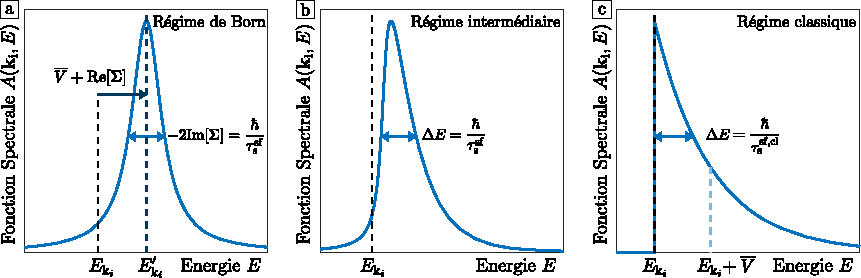
\includegraphics[width=\textwidth]{Fig/TauS_NJP/illustration_fonction_spectrale_diffusion.pdf}
\caption{\textbf{Illustration du profil de la fonction spectrale dans les différents régimes de diffusion.} \textbf{a.} Dans la limite d'un désordre faible, la self-energy est approximativement constante autour de l'énergie cinétique. La forme de la fonction spectrale est alors lorentzienne, dont la largeur est donnée par la partie imaginaire de la self-energy, inversement proportionnelle au temps de diffusion élastique $\taus^{\mathrm{sf}}$. \textbf{b.} Fonction spectrale dans le régime intermédiaire, pour lequel aucune prédiction générale n'existe. On peut néanmoins définir un temps de diffusion élastique effectif $\taus^{\mathrm{sf}}$ à l'aide de la largeur de la fonction spectrale. \textbf{c.} Dans la limite classique d'un désordre très fort, la fonction spectrale converge vers la distribution de potentiel décalée de l'énergie cinétique initiale. Cette situation est illustrée ici pour un speckle répulsif.}
\label{fig:illustration_fonction_spectrale_diffusion}
\end{figure}


\paragraph*{Lien entre la fonction spectrale et la décroissance de l'état initial}
Il est possible de déterminer d'autres expressions de la fonction spectrale en revenant à la définition de la fonction de Green \ref{eq:definition_green}. Notamment, on peut montrer que
\begin{equation}
A(\mathbf{k}_{\mathrm{i}},E)=-\frac{1}{\pi} \overline{\langle \mathbf{k}_{\mathrm{i}} | \mathrm{Im}\left[G(E)\right]| \mathbf{k}_{\mathrm{i}} \rangle} = \overline{\langle \mathbf{k}_{\mathrm{i}} | \delta(E-\hat{H})|\mathbf{k}_{\mathrm{i}}\rangle} \text{ ,}
\end{equation}
en utilisant la relation $ 1/(x+i0^+)=\mathrm{vp}(1/x)-i\pi \delta(x)$. 

En utilisant la représentation exponentielle de la distribution de Dirac, on peut alors montrer que l'opérateur évolution moyen $\overline{U}_{\mathrm{k}_i}$ de l'état initial est simplement donné par la transformée de Fourier de la fonction spectrale
\begin{equation}
\overline{U}_{\mathrm{k}_{\mathrm{i}}}(t)=\left\langle \mathbf{k}_{\mathrm{i}} | \overline{\exp(-itH)}  | \mathbf{k}_{\mathrm{i}} \right\rangle = \int{\diff E e^{-iEt} A(\mathbf{k}_{\mathrm{i}},E)} \text{ .}
\end{equation}
Un tel résultat n'a rien de surprenant. En effet, l'allumage brusque du désordre sur les atomes projette l'état initial sur les états d'énergie propre du désordre, dont la distribution d'énergie est donnée par la fonction spectrale en vertu de la formule \ref{eq:fonction_spectrale}. L'évolution temporelle de l'état initial est donc naturellement donnée par la transformée de Fourier de cette distribution d'énergie, c'est à dire la fonction spectrale. 

Dans la continuité de l'image physique selon laquelle le temps de diffusion élastique correspond au temps de vie de l'état initial $\etat{\mathbf{k}_{\mathrm{i}}}$ dans le désordre, il est possible de définir un temps caractéristique $\taus^{\mathrm{sf}}$ basé sur la largeur de la distribution d'énergie. On définit ainsi $\Delta E = \hb/\taus^{\mathrm{sf}}$ avec $\Delta E$ la largeur totale à mi-hauteur de la fonction spectrale tel qu'illustré dans la figure \ref{fig:illustration_fonction_spectrale_diffusion}. 

\subsection{Approximation de Born: premier ordre}
expansion de Born.
\begin{equation}
\Sigma(E,\mathbf{k}_{\mathrm{i}}) = \sum_{n=1}^{+\infty}{\overline{\left\langle \mathbf{k}_{\mathrm{i}}\left| \hat{V} \left(\hat{G}_0(E) \hat{V}\right)^n \right|\mathbf{k}_{\mathrm{i}}\right\rangle}}
\end{equation}


\begin{equation}
\Sigma=\Sigma^{(1)}+\Sigma^{(2)} + \cdots
\end{equation}
avec $\Sigma^{(1)}=\overline{V G_0 V}$ et $\Sigma^{(2)}=\overline{V G_0 V G_0 V}$.

\begin{equation}
A(\mathbf{k}_{\mathrm{i}},E)= \frac{1}{\pi} \frac{\Delta E/2}{(\Eki - \Eki')^2+\Delta E^2/4}
\end{equation}
avec $\Delta E=-2 \mathrm{Im}[\Sigma^{(1)}(\Eki,\mathbf{k}]_{\mathrm{i}})]$ et $\Eki'=\Eki+\overline{V}+\mathrm{Re}[\Sigma^{(1)}(\Eki,\mathbf{k}_{\mathrm{1}})]$

\begin{equation}
\frac{\hb}{\taus^{\mathrm{sf}}}=-2 \mathrm{Im}[\Sigma^{(1)}(E_{\mathrm{k}_i},\mathbf{k}_{\mathrm{i}})]=2\pi \sum_{\mathbf{k}'}{\widetilde{C}(\mathbf{k}'-\mathbf{k}_{\mathrm{i}}) \delta(E_{\mathrm{k}'}-E_{\mathrm{k}_i})}
\end{equation}

\begin{figure}
\centering
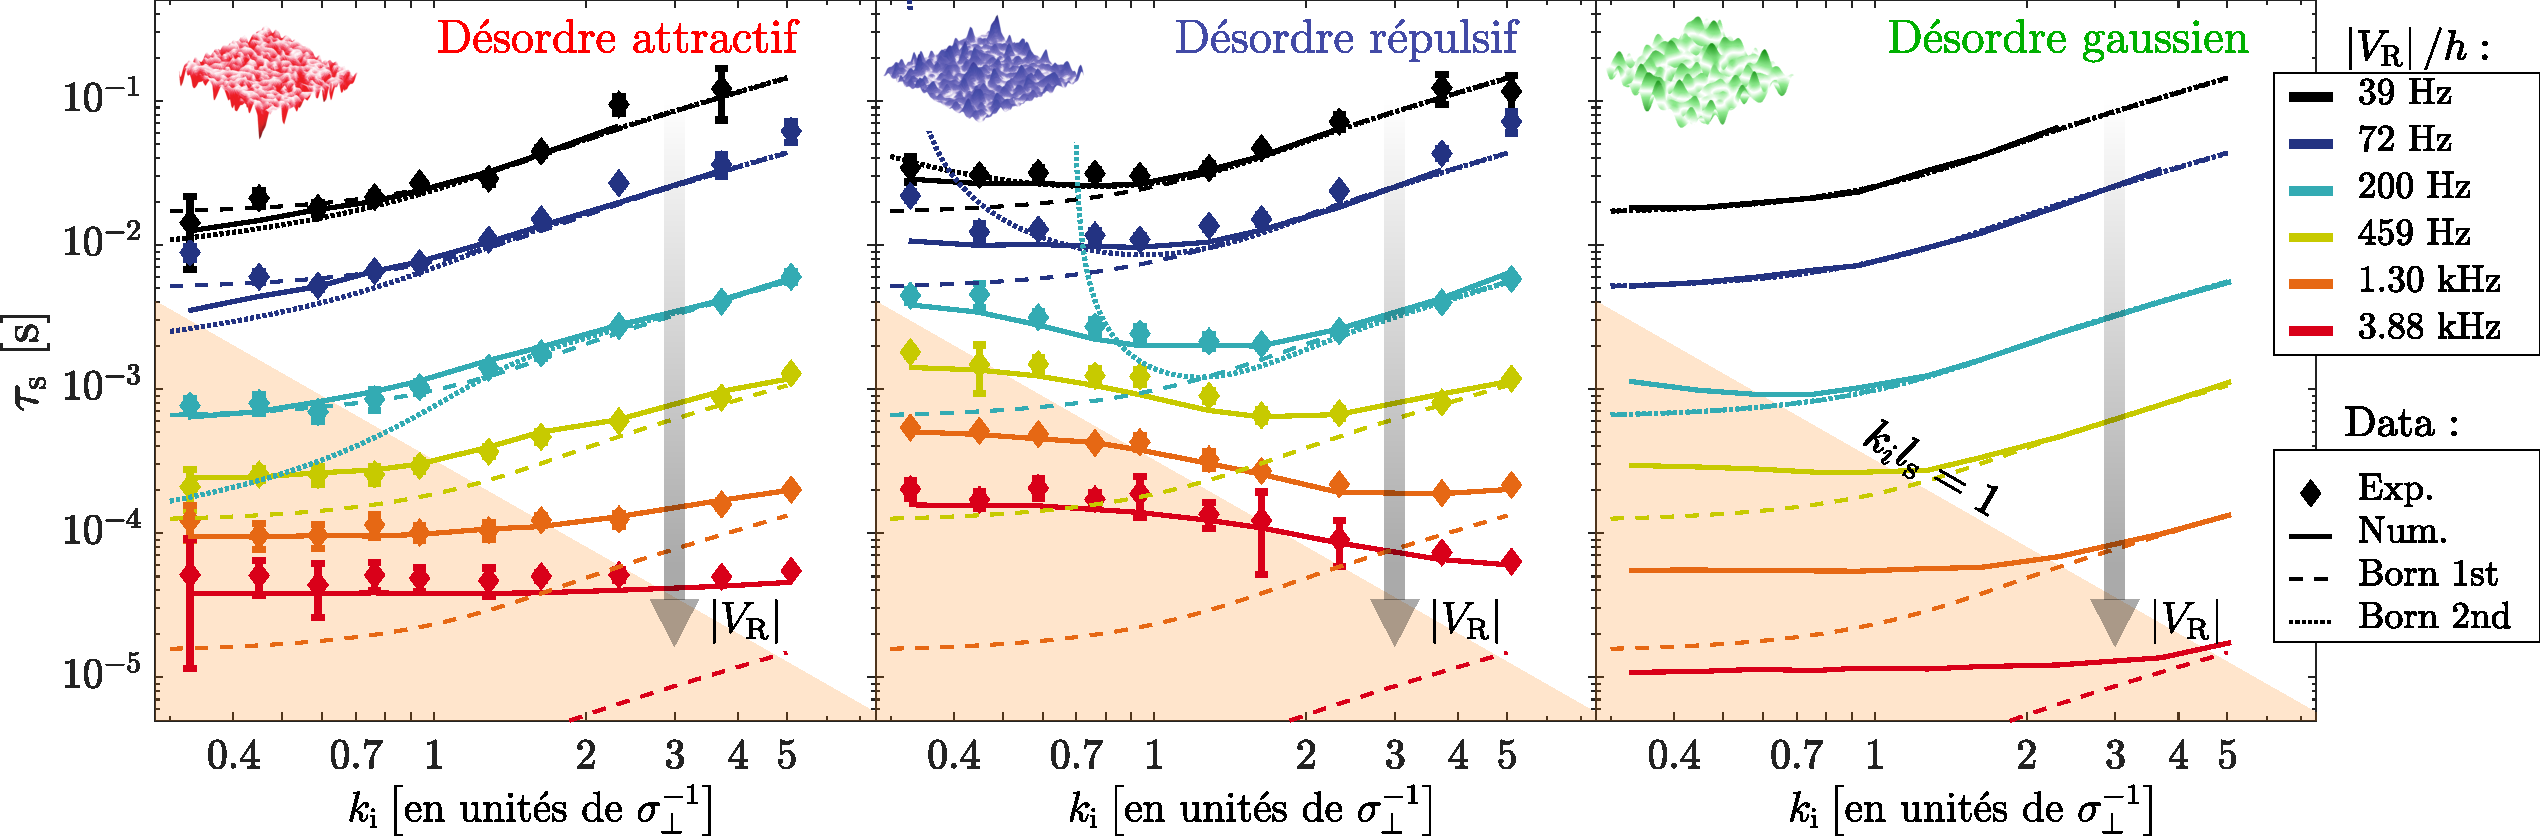
\includegraphics[width=\textwidth]{Fig/TauS_NJP/donnees_taus_ordre3.pdf}
\caption{\textbf{Données expérimentales et numériques du temps de diffusion élastique.} Stuff.}
\label{fig:donnees_taus_ordre_3}
\end{figure}


\subsection{Approximation de Born: second ordre}
\subsection{Approximation de Born auto-consistante}
\begin{equation}
\Sigma_{\mathrm{scba}}(E,\mathbf{k}_{\mathrm{i}})=\widetilde{C}(\mathbf{k}_{\mathrm{i}})\ast \overline{G}_{\mathrm{scba}}(E,\mathbf{k}_{\mathrm{i}})
\end{equation}
\begin{equation}
\overline{G}_{\mathrm{scba}}(E,\mathbf{k}_{\mathrm{i}}) = \frac{1}{E-E_{\mathrm{k}_i} - \overline{V} - \Sigma_{\mathrm{scba}}(E,\mathbf{k}_{\mathrm{i}})}
\end{equation}

\section{Temps de diffusion élastique et fonctions spectrales mesurées pour un désordre de type speckle}
\subsection{Limite de l'approche auto-consistante pour un désordre de type speckle}
\subsection{Mesure des fonctions spectrales}
\subsection{Comparaison du temps de diffusion élastique avec les fonctions spectrales mesurées}
